\documentclass[12pt]{article}

\usepackage{amsmath}
\usepackage{graphicx}
\usepackage{hyperref}
\usepackage{cite}
\usepackage[margin=1.2in]{geometry}

\providecommand{\eqn}[1]{eqn.~(\ref{eqn:#1})}
\providecommand{\tab}[1]{Table~\ref{tab:#1}}
\providecommand{\fig}[1]{Figure~\ref{fig:#1}}

\title{Evolution of ELG Signal-to-Noise Ratio\\
with DESI Model\\
\vspace{5mm}{\large\bf DESI-doc-3977-v1}}
\author{David Kirkby}

\begin{document}
\maketitle

\noindent {\bf Version History:}
\begin{itemize}
    \item v1: Changes from desimodel 0.3.1 (CDR) - 0.9.5 (Nov 2017) - 0.9.6 (Jun 2018) using specsim v0.13.
\end{itemize}

\section{Introduction}

This note defines a methodology to track changes in the signal-to-noise (SNR) ratio of a representative sample of DESI emission-line galaxy (ELG)
targets using spectral simulations, and documents its evolution with changes to the DESI model.  We focus on the SNR of ELGs
since they are the faintest objects targeted by DESI, so drive the dark- and gray-time survey operations strategy and expected performance,
as embodied in the level-3 science requirement L3.1.3:
\begin{quote}
\it The median S/N= 7 flux limit will be 10., 9, 9, 8, and $9\times 10^{−17}$ erg cm$^{-2}$ s$^{-1}$
in redshift bins of 0.6-0.8, 0.8-1.0, 1.0-1.2, 1.2-1.4 and
1.4-1.6 for an [OII] doublet emission line in an ELG galaxy with
an exponential half-light radius of 0.45 arcsec observed in 1.1 arcsec
seeing with the sky spectrum under median, dark-sky, photometric
conditions.
\end{quote}
DESI-867\cite{desi-867} describes the methodology and results used for the Conceptual Design Report (CDR) in 2014.
This note describes some updates to the methodology and tracks changes in the results since the CDR.

The latex source for this note is maintained in {\tt /doc/tex/desi3977/} of the {\tt desimodel} package on github,
with an accompanying juypter notebook in {\tt /doc/nb/ELG-SNR.ipynb}. This version of the document corresponds to
version {\tt 0.9.7} of the {\tt desimodel} package and version {\tt v0.13} of the {\tt specsim} package.

\section{Methodology}

This section describes the methodology used to estimate ELG SNR, highlighting updates since the CDR.

\subsection{Emission Line Galaxy Model}

We use the reference ELG spectrum tabulated in:
\begin{quote}
{\tt \$DESIMODEL/data/spectra/\\
spec-elg-o2flux-8e-17-average-line-ratios.dat}
\end{quote}
and described in Section 2.3 of DESI-867-v1\cite{desi-867}. This spectrum consists of only the following emission lines:
\begin{itemize}
    \item The doublet [OII](3727 \AA) and [OII](3730 \AA),
    \item H-$\beta$,
    \item the doublet [OIII](4960 \AA) and [OIII](5008 \AA), and
    \item H-$\alpha$.
\end{itemize}
Continuum is omitted since we are primarily interested in how well
the [OII] doublet can be identified and measured.  The emission line parameters are taken from Section 2.3 of DESI-867-v1 and also listed
in \tab{elg-params}. Note that the [OII] integrated flux specifies the normalization of each peak in this parameterization.

\begin{table}[htb]
\begin{center}
\begin{tabular}{lr}
    Description & Value \\
    \hline
    Integrated [OII] doublet flux & $8\times 10^{-17}$ erg cm$^{-2}$ s$^{-1}$ \\
    Ratio 3730 / 3727 of the [OII] doublet integrated fluxes & 1.37 \\
    Ratio [OII] / H-beta of integrated fluxes & 2.5 \\
    Ratio 5008 / H-beta of integrated fluxes & 1.6 \\
    Ratio 5008 / 4960 of the [OIII] doublet integrated fluxes & 2.984 \\
    Ratio H-$\alpha$ / H-$\beta$ of integrated fluxes & 3.0 \\
    \hline
    Rest wavelength of the bluer [OII] doublet peak & 3727.092 \AA \\
    Rest wavelength of the redder [OII] doublet peak & 3729.875 \AA \\
    Rest wavelength of the H-$\beta$ peak & 4862.708 \AA \\
    Rest wavelength of the bluer [OIII] doublet peak & 4960.295 \AA \\
    Rest wavelength of the redder [OIII] doublet peak & 5008.240 \AA \\
    Rest wavelength of the H-$\alpha$ peak & 6564.603 \AA \\
    \hline
\end{tabular}
\caption{Nominal ELG emission-line parameters used in this note, originally from DESI-867-v1 Section 2.3.}
\label{tab:elg-params}
\end{center}
\end{table}

All lines are assumed to have the same velocity dispersion of $\sigma_v 70$ km/s, with a lineshape given by:
$$
f(\lambda; F_0, \lambda_0) = \frac{F_0}{\sqrt{2\pi}\,\lambda\,\sigma_{\log}}\, \exp\left[
-\frac{1}{2}\left( \frac{\log_{10}\lambda - \log_{10}\lambda_0}{\sigma_{\log}}\right)^2\right]\; ,
$$
where
$$
\sigma_{\log} \equiv \frac{\sigma_v}{c \log 10} \; ,
$$
and $F_0$ and $\lambda_0$ are the line's integrated flux and central wavelength, respectively.

\subsection{DESI Emission Line Galaxy Sample}

We assume the distribution of ELG target redshifts specified in:
\begin{quote}
{\tt \$DESIMODEL/data/targets/nz\_elg.dat}
\end{quote}  
which uses bins of $\Delta z = 0.1$ covering $0.6 \le z < 1.7$ as shown in \fig{elg-sample}.
Note that with $z \ge 0.6$, the H-$\alpha$ is never detected. 

\begin{figure}[htb]
\begin{center}
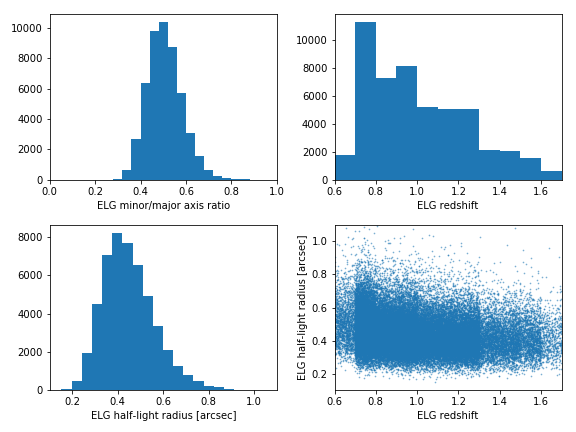
\includegraphics[width=6in]{elg-sample}
\caption{Distribution of ELG redshift and profile size and shape used in this note. The mean half-light radius is 0.45 arcseconds.
The median minor-to-major axis ratio is 0.5.}
\label{fig:elg-sample}
\end{center}
\end{figure}

We assume an exponential (Sersic $n=1$) galaxy profile with a mean half-light radius of 0.45 arcseconds. Profiles are also specified
by an ellipticity (minor-to-major axis ratio, with median value 0.5) and position angle on the sky. The assumed (uncorrelated)
distributions of half-light radius and ellipticity
are shown in \fig{elg-sample} and roughly matched to distributions of corresponding catalog quantities from the DESI image survey.
The half-light radius is assumed to scale with inverse luminosity distance, calculated using a Planck 2015 cosmology. The position angle
distribution is uniform. Code to sample these distributions is provided in {\tt /doc/nb/ELG-SNR.ipynb}.

\subsection{Spectral Simulation}

We use the {\tt specsim} package version {\tt v0.13} to simulate the expected SNR, with the following main ingredients:
\begin{itemize}
    \item Instrument model corresponding to version {\tt 0.9.6} of {\tt desimodel}:
    \begin{itemize}
        \item CCD dark current and read noise.
        \item Sky to CCD throughput, excluding fiber acceptance.
        \item Blur and radial offset as a function of wavelength and focal-plane radius.
    \end{itemize}
    \item Fiber acceptance fraction calculated assuming~\cite{desi-2720}:
    \begin{itemize}
        \item Instrumental blur and radial offsets.
        \item A fixed atmospheric seeing of 1.1 arcseconds full-width half maximum.
        \item Varying radial and azimuthal plate scales.
        \item Realistic galaxy size and shape distributions.
    \end{itemize}
    \item Nominal dark sky surface brightness tabulated in
    \begin{quote}
        {\tt \$DESIMODEL/data/spectra/spec-sky.dat}
    \end{quote}
\end{itemize}
We simulate a 1000 second exposure during nominal dark conditions with 100 fibers randomly distributed over the focal plane and observing the identical ELG spectrum
described above at a fixed redshift.  An outer loop steps through redshifts in the range $0.5 \le z < 1.6$, using $\Delta z = 0.002$ steps,
and computes the mean expected signal and noise at each fiber, in 0.5~\AA pixels.

The {\tt specsim} package implements several different schemes for computing fiber acceptance fractions.  The {\tt galsim} method is the most accurate and flexible, but
also the slowest.  The default {\tt fastsim} mode interpolates pre-computed {\tt galsim} results.  For the calculations described here, the {\tt fastsim} mode is roughly
a factor of two faster but over-estimates the fiber acceptance fraction (and therefore the signal) by about 1\%. The reason for this is that we assume a
distribution of minor / major axis ratios with a median of 0.5, but the pre-computed results assume a fixed ratio of 0.7.  We use {\tt galsim}
results consistently in this note (except for the CDR baseline), to avoid the (small) approximation errors inherent to the {\tt fastsim} mode.

\subsection{Figures of Merit}

We define the total SNR of the [OII] doublet as the quadrature sum over all 0.5~\AA pixels of each spectrograph (b,r,z) with a wavelength:
\begin{equation}
    3715~\AA < \frac{\lambda}{1 + z} < 3742~\AA \; .
\end{equation}
This results in a single number per fiber and per redshift. \fig{results-baseline} shows the results for the baseline DESI configuration.
We reduce the [OII] SNR versus redshift to a single weighted averaged using $n(z)$ weights derived from the expected redshift
distribution of DESI ELG targets (see \tab{results-summary}).

\begin{figure}[htb]
\begin{center}
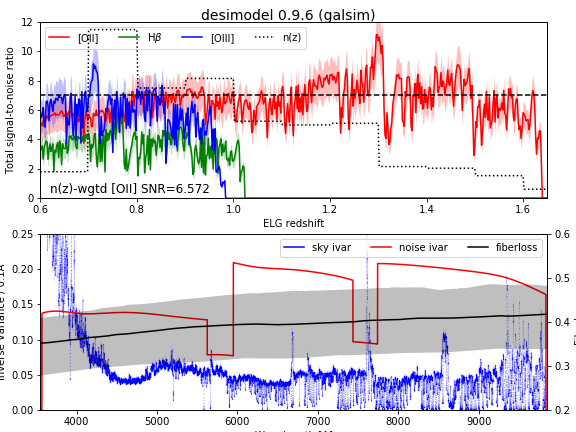
\includegraphics[width=6in]{results-baseline}
\caption{Results for the baseline DESI configuration. Shaded bands show 5--95 percentile ranges and solid curves show medians (both over fibers).
The upper plot shows SNR versus redshift for the [OII], H-$\beta$ and [OII] emission lines. The lower plot shows the sky and noise inverse variance
(quadrature summed over cameras, per 0.1~\AA, left axis) and fiberloss (at $z=1.2$, right axis) versus wavlength.}
\label{fig:results-baseline}
\end{center}
\end{figure}

In order to compare directly with the science requirement L3.1.3, we also calculate an integrated [OII] flux limit to acheive $\text{SNR}_0 = 7$ as:
$$
F_{\text{lim}}(z) = F_0\,\frac{\text{SNR}_0}{SNR(z)} \; ,
$$
where $\text{SNR}(z)$ is the median [OII] SNR (over fibers) at each redshift simulated with the nominal flux $F_0 = 8\times 10^{-17}$ erg cm$^{-2}$ s$^{-1}$.
We then take the median of $F_{\text{lim}}(z)$ in the bins
of width $\Delta z = 0.2$ specified in the requirement. These values are summarized in \tab{results-summary} and show that the expected performance has
been quite stable since the CDR, as engineering parameters have been refined and simulation realism has increased.

\section{SNR Evolution}

\begin{table}[htb]
\begin{center}
\begin{tabular}{lrrrrrr}
    DESIMODEL     & Weighted  & \multicolumn{5}{c}{[OII] Flux Limit ($\times 10^{-17}$ erg cm$^{-2}$ s$^{-1}$)} \\
    Configuration & [OII] SNR & 0.6--0.8 & 0.8--1.0 & 1.0--1.2 & 1.2--1.4 & 1.4--1.6 \\
    \hline
    0.9.6            &  6.572 &  9.9 &  8.1 &  8.6 &  7.5 &  8.2 \\
    0.9.5 +thru+blur &  6.463 & 10.0 &  8.2 &  8.7 &  7.6 &  8.3 \\
    0.9.5 +thru      &  6.419 & 10.1 &  8.3 &  8.8 &  7.7 &  8.4 \\
    0.9.5            &  6.565 & 10.0 &  8.1 &  8.6 &  7.4 &  8.3 \\
    0.3.1 (CDR)      &  6.262 & 10.1 &  8.6 &  8.9 &  7.6 &  8.3 \\
    \hline
    Requirement      &     -- & $\le 10$ & $\le 9$ & $\le 9$ & $\le 8$ & $\le 9$ \\
    \hline
\end{tabular}
\caption{Summary of SNR figures of merit described in the text for different simulated configurations.
The changes between 0.9.5 and 0.9.6 are broken down into the cummulative effects of updating the throughput, blur, and noise,
i.e., {\tt 0.9.6 = 0.9.5 +thru +blur +noise}.  CDR results are estimated from SNR curves stored with
Reference~\cite{desi-867} (see {\tt /doc/nb/ELG\_SNR.ipynb} for details.)}
\label{tab:results-summary}
\end{center}
\end{table}

The flowdown of engineering data to the simulations is primarily through DESI-347\cite{desi-347}, which summarizes
the project's systems engineering throughput, noise, and SNR calculations.  The current version {\tt v13} was released on 26-Jun-2018,
and contains the following updates since {\tt v12} of 27-Nov-2017 (see {\tt desimodel} issue \#88 for plots and details\footnote{
\url{https://github.com/desihub/desimodel/issues/88}}):
\begin{itemize}
    \item Throughput uses updated C2 surfaces and includes ADC surfaces for the first time.
    \item Several contributions to achromatic blur estimates updated, resulting in slightly lower blurs overall.
    \item CCD noise and dark currents updated. Note that {\tt desimodel} versions before {\tt 0.9.6} were not correctly
    tracking the noise levels in DESI-347 versions prior to {\tt v13}.
\end{itemize}

The DESI Conceptual Design Report (CDR) used {\tt desimodel} version {\tt 0.3.1} and an early version of {\tt specsim}.
The current {\tt specsim} implements a more detailed spectral simulation, which requires more detailed input assumptions.
Specifically, we now model expected variations of the fiber acceptance fraction over the focal plane due to:
\begin{itemize}
    \item The radial and azimuthal plate scales varying with focal-plane radial position.
    \item Variations of the fiber acceptance fraction over the focal plane due to:
    \begin{itemize}
        \item Variations in the galaxy size and shape.
        \item Chromatic abberations in the design optics leading to instrumental blur and centroid offsets.
    \end{itemize}
\end{itemize}
For comparison, the CDR used a fixed ELG fiber acceptance versus wavelength that assumed a round profile
with 0.45 arcsecond half-light radius.

\bibliographystyle{unsrt}
\bibliography{elgsnr}

\end{document}
